%%%%%%%%%%%%%%%%%%%%%%%%%%%%%%%%%%%%%%%%%%%%%%%%%%%%%%%%%%%%%%%%%%%%%%
% How to use writeLaTeX: 
%
% You edit the source code here on the left, and the preview on the
% right shows you the result within a few seconds.
%
% Bookmark this page and share the URL with your co-authors. They can
% edit at the same time!
%
% You can upload figures, bibliographies, custom classes and
% styles using the files menu.
%
%%%%%%%%%%%%%%%%%%%%%%%%%%%%%%%%%%%%%%%%%%%%%%%%%%%%%%%%%%%%%%%%%%%%%%

\documentclass[12pt]{article}

\usepackage{multirow}
\usepackage{xcolor}


\usepackage{sbc-template}

\usepackage{graphicx,url}

%\usepackage[brazil]{babel}   
\usepackage[utf8]{inputenc}  

     
\sloppy

\title{Detecção de eixos de caminhões}

\author{Matheus Peixoto Ribeiro Vieira - 22.1.4104}


\address{Departamento de Computação (DECOM) -- Universidade Federal de Ouro Preto (UFOP)
  \email{matheus.peixoto@aluno.ufop.edu.br}
}

\begin{document} 

\maketitle

\begin{abstract}
    Road transportation in Brazil features a large number of heavy vehicles in circulation, which can cause excessive wear and tear on the roads. In this context, the implementation of effective techniques to monitor the traffic of these vehicles becomes essential. Many cities impose restrictions not only based on the total gross weight but also considering the number of axles. In this regard, convolutional neural networks emerge as a promising tool for identifying the number of axles of heavy vehicles through images. This study aims to explore the use of these techniques to address the issue of vehicle monitoring and classification, contributing to the preservation of public roads.
\end{abstract}
     
\begin{resumo} 
    O transporte rodoviário no Brasil apresenta uma grande quantidade de veículos pesados em circulação, o que pode causar desgastes excessivos nas estradas. Nesse contexto, torna-se essencial a implementação de técnicas eficazes para fiscalizar o trânsito desses veículos. Muitas cidades adotam restrições não apenas com base no peso bruto total, mas também considerando a quantidade de eixos. Nesse sentido, as redes neurais convolucionais surgem como uma ferramenta promissora para identificar a quantidade de eixos de veículos pesados por meio de imagens. Este trabalho tem como objetivo explorar o uso dessas técnicas para solucionar o problema de fiscalização e classificação de veículos, contribuindo para a preservação das vias públicas.
\end{resumo}


\section{Introdução}
    Segundo o Conselho Nacional de Trânsito (CONTRAN), o transporte de cargas em veículos pesados está sujeito a limites para o Peso Bruto Total Combinado (PBTC), que corresponde à soma do peso do veículo, sua carroceria e a carga transportada. Assim, veículos de três eixos do tipo semirreboque podem atingir um PBTC máximo de 25,5 toneladas, e veículos de quatro eixos têm limite de até 58,5 toneladas \cite{resolucao_contran}.
    
    Veículos com um maior peso exercem um impacto significativo sobre as condições do pavimento, acelerando sua deterioração ao longo do tempo, levando a danos às estradas em trechos rodoviários \cite{damage_on_roads}.
    
    Para mitigar esses impactos, diversas cidades brasileiras adotam restrições à circulação de veículos pesados em áreas urbanas, com o objetivo de preservar a infraestrutura viária. Um exemplo disso ocorreu em Coronel Fabriciano, Minas Gerais, onde o Decreto Municipal nº 8.472/2023 proibiu a passagem de veículos com peso bruto total acima de 23 toneladas, bem como daqueles com mais de três eixos, em vias de quatro bairros específicos \cite{prefeitura_de_coronel_fabriciano}. Da mesma forma, em Ouro Branco, Minas Gerais, a Lei Municipal nº 2.794/2024 restringe a circulação de veículos de carga com três ou mais eixos em áreas de patrimônio histórico, proteção ambiental, unidades de conservação e outros locais determinados, salvo em casos de autorização prévia \cite{lei_ourobranco_2024}.
    
    Para auxiliar na fiscalização do trânsito em diferentes áreas, este trabalho explora a hipótese de que redes neurais convolucionais podem ser utilizadas para identificar a quantidade de eixos dos veículos. Essa abordagem é fundamentada no fato de que essas redes já demonstraram excelentes resultados na identificação de diferentes classes de veículos, conforme apresentado em \cite{iluminacao_adversa}, e na contagem de eixos, conforme explorado em \cite{marcomini2023truckaxledetectionconvolutional}.

\section{Trabalhos relacionados}

    Os caminhões podem variar em tamanho, tipo de carga e configuração da cabine. Para classificar essas características, \cite{Almutairi2022} utilizou imagens laterais de veículos capturadas pelo Departamento de Transporte da Flórida. O estudo, focado na classificação do tipo de caminhão com base nos critérios da Federated Highway Administration, alcançou 89\% de acurácia no conjunto de testes usando o modelo Inception V3.

    Nem sempre as condições de iluminação são propicias, e, levando este fator em consideração, \cite{iluminacao_adversa} criou um dataset com condições de iluminação adversas para classificar tipos de veículos. O treinamento envolveu diferentes modelos com redes convolucionais pré-treinadas, obtendo melhores resultados com uma ResNet, atingindo um resultado de 99.68\%.

    Mesmo possuindo imagens laterais, nem sempre elas obterão uma visão completa dos veículos, que podem não caber por completo na imagem. Dessa forma, \cite{Souza2024} propôs um algoritmo para reconstruir uma imagem com diferentes quadros de um vídeo a partir da passagem de um veículo. Em seguida, utilizando o YOLO foi detectado a quantidade de eixos dos veículos que estavam passando, obtendo melhores resultados com o YOLOv5m.

    Além de se preocupar com a contagem de eixos, \cite{Miles2022} também se preocupou com a velocidade dos veículos, ao mesmo tempo que se preocupava com a não visibilidade dos eixos de todos os veículos. Dessa forma, utilizando a YOLOv4 e ignorando veículos que não era possível identificar todos os eixos, foi obtido um mAP de 93.3\% nas imagens de teste.

    Por fim, \cite{marcomini2023truckaxledetectionconvolutional} decidiu investigar diferentes arquiteturas para a detecção exclusiva de eixos a partir de imagens coletadas em rodovias no Brasil, avaliando modelos de Fast R-CNN, diferentes versões do YOLOv3 e uma rede neural Single Shot Detector (SSD). Assim, os modelos YOLOv3-spp e SSD-ssd300 obtiveram os melhores resultados ao calcular o F1-score, obtendo uma pontuação de 0.98.

\section{Metodologia}

    Esta seção descreve a metodologia proposta para este trabalho, sendo dividida em quatro partes: (1) Base de dados; (2) Pré-processamento; (3) Características dos modelos implementados \& (4) Métricas de avaliação. 

    \subsection{Base de dados}
        Entre os artigos mencionados, observa-se que as bases de dados utilizadas são, em sua maioria, privadas e destinadas a objetivos específicos. Um exemplo é apresentado em \cite{Miles2022}, onde os dados foram fornecidos por uma empresa particular, sendo o desenvolvimento do projeto direcionado para uma aplicação específica desses dados.
        
        Por outro lado, em \cite{marcomini2023truckaxledetectionconvolutional}, os próprios autores destacam como principal contribuição do projeto a disponibilização de um \textit{dataset} contendo 382 imagens rotuladas, que identificam as posições de 1303 eixos de caminhões. Embora o número de imagens seja limitado, ele é suficiente para estudos iniciais de técnicas de detecção. Além disso, o uso de técnicas de \textit{data augmentation} pode ampliar a quantidade de dados disponíveis, aumentando a robustez dos modelos desenvolvidos.
        
        As imagens do \textit{dataset} foram capturadas lateralmente, oferecendo uma visão sem obstruções dos eixos dos veículos, como ilustrado em \ref{fig:caminhaoExemplo}. Todas as imagens foram registradas sob luz natural, de modo que o \textit{dataset} não inclui exemplos capturados durante o período noturno.

        \begin{figure}[ht]
            \centering
            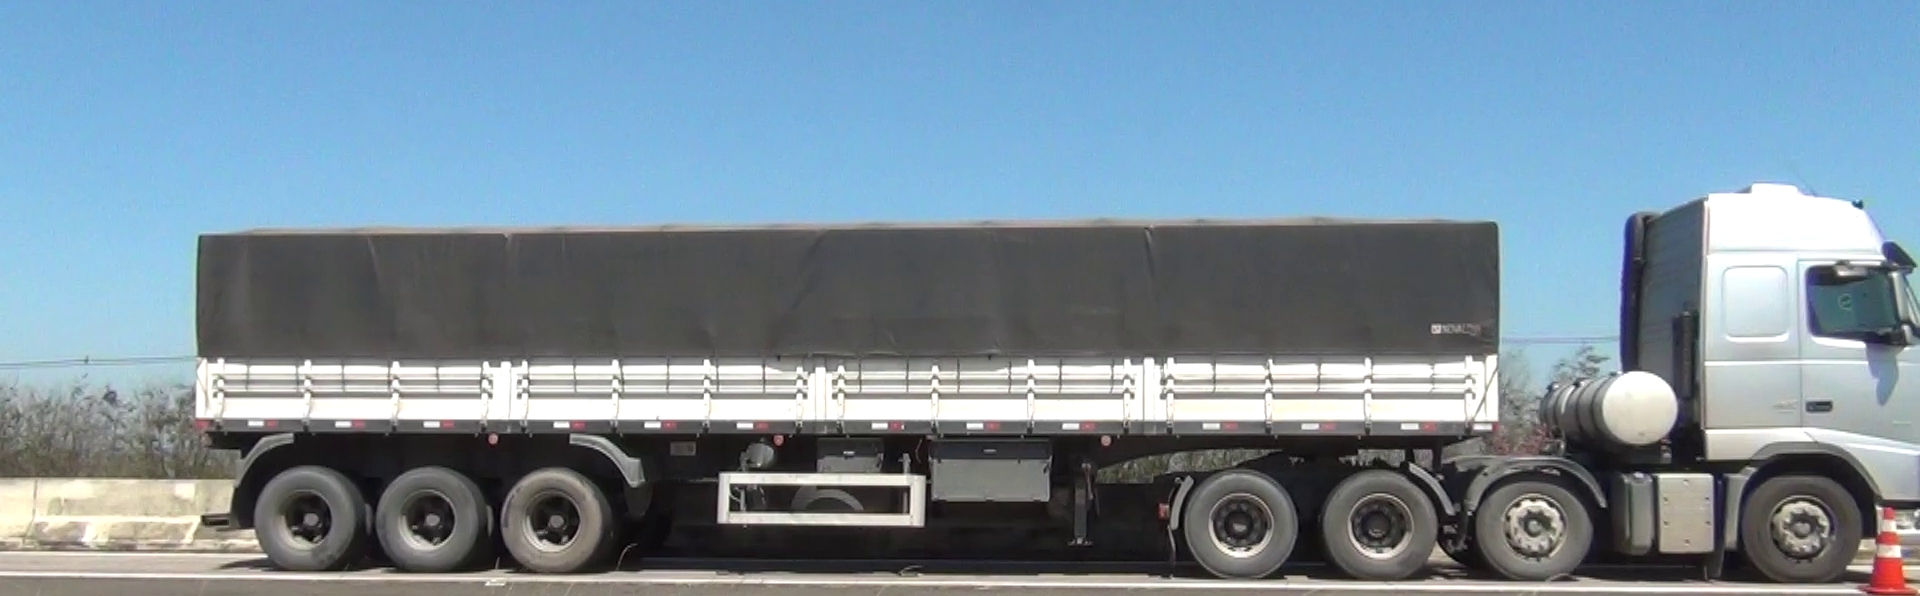
\includegraphics[width=.75\textwidth]{Images/20160927102749_color-[ROI-1]-1.jpg}
            \caption{Exemplo de imagem de caminhão}
            \label{fig:caminhaoExemplo}
        \end{figure}

    \subsection{Pré-processamento}

        Ao explorar o dataset compartilhado pelos autores, foi identificada uma quantidade maior de imagens do que a utilizada originalmente por eles, totalizando 725 imagens. No entanto, essas imagens não possuíam as anotações das localizações dos eixos.
        
        Para solucionar esse problema, utilizou-se a ferramenta Roboflow para realizar a identificação manual dos eixos. Posteriormente, as imagens foram divididas em três conjuntos: 70\% para treino, 15\% para avaliação e 15\% para teste.
        
        Nas imagens destinadas ao treino, foi aplicado um processo de data augmentation, incluindo giros horizontais e verticais, conversão de 15\% das imagens para tons de cinza, ajustes no brilho em 15\% das imagens e variações na exposição em 10\%. Além disso, foram adicionados efeitos de borrão com intensidade de 0,7 px e ruído de até 1,5\%. Com essas técnicas, o conjunto de dados passou a contar com 1.521 imagens para treino, 109 para avaliação e 109 para teste, onde todas foram redimensionadas para as dimensões 640x640.
        
        Essas modificações visam tornar o modelo mais robusto, permitindo um aprendizado mais eficiente das características dos eixos e, consequentemente, a realização de predições mais precisas.

    \subsection{Características do modelo implementado}
        Para este estudo, serão exploradas duas abordagens distintas. A primeira baseia-se nos trabalhos de \cite{Souza2024}, \cite{marcomini2023truckaxledetectionconvolutional} e \cite{Miles2022} para a detecção de eixos, utilizando as duas versões mais recentes do YOLO. A YOLOv11 \cite{khanam2024yolov11overviewkeyarchitectural} apresenta uma redução de 2\% no tempo de predição em comparação à YOLOv10 e possui 22\% menos parâmetros do que a YOLOv8m, tornando-se mais eficiente sem comprometer os níveis de acurácia. Já a YOLOv12 \cite{tian2025yolov12attentioncentricrealtimeobject} substitui as redes convolucionais por mecanismos de atenção, resultando em um tempo de latência inferior ao de seus antecessores.

        Já a outra abordagem será a de uma rede neural convolucional, como a utilizada em \cite{Almutairi2022}, porém sua saída será a quantidade de eixos presentes na imagem. Todavia, como a quantidade de eixos varia de acordo com o tipo de caminhão e não há uma distribuição balanceada para a quantidade de eixos, o uso de um classificador pode não gerar bons resultados. Assim, será feito um trabalho de regressão a fim de identificar a quantidade de eixos presentes na imagem.

    \subsection{Métricas de avaliação}
        Para os modelos baseados em YOLO, a métrica mAP (mean Average Precision) será utilizada para avaliar a qualidade das predições e sua correspondência com as anotações originais. Quanto maior o valor da mAP, mais precisas e alinhadas com o esperado serão as predições do modelo.
        
        Serão consideradas diferentes variações da mAP, como mAP50, mAP75 e mAP50-95. Essas variações indicam a precisão das detecções com base no limiar de IoU (Interseção sobre União). A mAP50 considera uma detecção correta quando a predição atinge pelo menos 50\% de IoU com a anotação real, enquanto a mAP75 exige um mínimo de 75\%. Já a mAP50-95 calcula a média da precisão em múltiplos limiares, variando de 50\% a 95\%, proporcionando uma visão mais abrangente do desempenho do modelo.

        Para os modelos treinados por meio de regressão, o valor real de cada predição será arredondado para o inteiro mais próximo e comparado com a sua \textit{label}. Dessa forma, serão utilizadas métricas de Precision (Indicando o quanto dos eixos identificados de fato eram eixos), Recall (Indicando quantas vezes o modelo não identificou um eixo onde de fato não deveria ter), F1-Score e acurácia para avaliar a qualidade dos modelos. 
        
        Os modelos treinados com YOLO também serão comparados com os outros, onde será utilizado a quantidade de eixos detectados para que se obtenha tais métricas, independente se o modelo identificou algo em um local errado. Consequentemente, seus resultados serão diferentes nas duas avaliações.       
    

\section{Experimentos e resultados}
    Para a execução dos experimentos, foi utilizado framework PyTorch, para a criação dos modelos, e do ultralytics, para o treinamento com a YOLO.
    
    \subsection{Modelo de detecção}
        Para a realização da detecção, optou-se pelos modelos YOLOv11m e YOLOv12m, treinados utilizando a biblioteca do Ultralytics. O treinamento foi conduzido por 25 épocas, com critério de paciência de cinco épocas. Tanto o otimizador quanto a taxa de aprendizado (\textit{learning rate}) seguiram os valores padrão da função de treinamento do YOLO.

        Após a conclusão do treinamento, os modelos foram avaliados nos dados de teste, e foram calculadas as métricas mAP, precisão, recall e F1-score para as predições. Os resultados obtidos estão apresentados na Tabela \ref{tab:yolo_results}.

        \begin{table}[!htb]
            \centering
            \begin{tabular}{| c | c | c | c | c | c | c | }
                 \hline
                 Modelo & mAP50 & mAP75 & mAP50-95  & Precisão & Revocação & F1 Score\\
                 \hline
                 YOLOv11m & 0.99  &  0.93 &  0.77     &   0.99    &  0.99  &  0.99\\
                 \hline
                 YOLOv12m & 0.99 & 0.94 & 0.77 & 0.99 & 0.99 & 0.99 \\
                 \hline
            \end{tabular}
            \caption{Resultados de teste da YOLO}
            \label{tab:yolo_results}
        \end{table}

        Com tais valores, percebe-se que os modelos identificaram, de forma excepcional, a presença dos eixos nas imagens, possuindo uma baixíssima taxa de falsos-positivo, como observado pela precisão, e uma alta detecção dos objetos, como mostra o recall, resultando em um ótimo valor para o F1-Score.

        No que se refere à localização dos eixos, observou-se que, ao permitir maior flexibilidade, os modelos conseguiram prever suas posições com maior precisão. Esse comportamento é evidenciado pelo resultado do mAP50-95, uma métrica mais rigorosa, que atingiu um valor de 0.77. No entanto, ao considerar uma margem de flexibilidade maior, verificou-se um aumento significativo na qualidade das predições, refletido no mAP75 (0.93 para a YOLOv11 e 0.94 para a YOLOv12) e no excepcional mAP50 (0.99).

        As predições realizadas pelo YOLOv11 podem ser observadas nas figuras \ref{fig:predicao_yolo_1}, \ref{fig:predicao_yolo_2} e \ref{fig:predicao_yolo_3}, sendo valores muito similares para a YOLOv12. Nota-se que o modelo identificou os eixos dos caminhões de forma bastante precisa. Entretanto, a confiança das predições situou-se em torno de 85\%, o que pode ter impactado o resultado do mAP50-95. Dessa forma, levanta-se a hipótese de que métricas ainda melhores poderiam ser alcançadas com anotações mais precisas e consistentes nas imagens de treinamento.

        \begin{figure} [!htb]
            \centering
            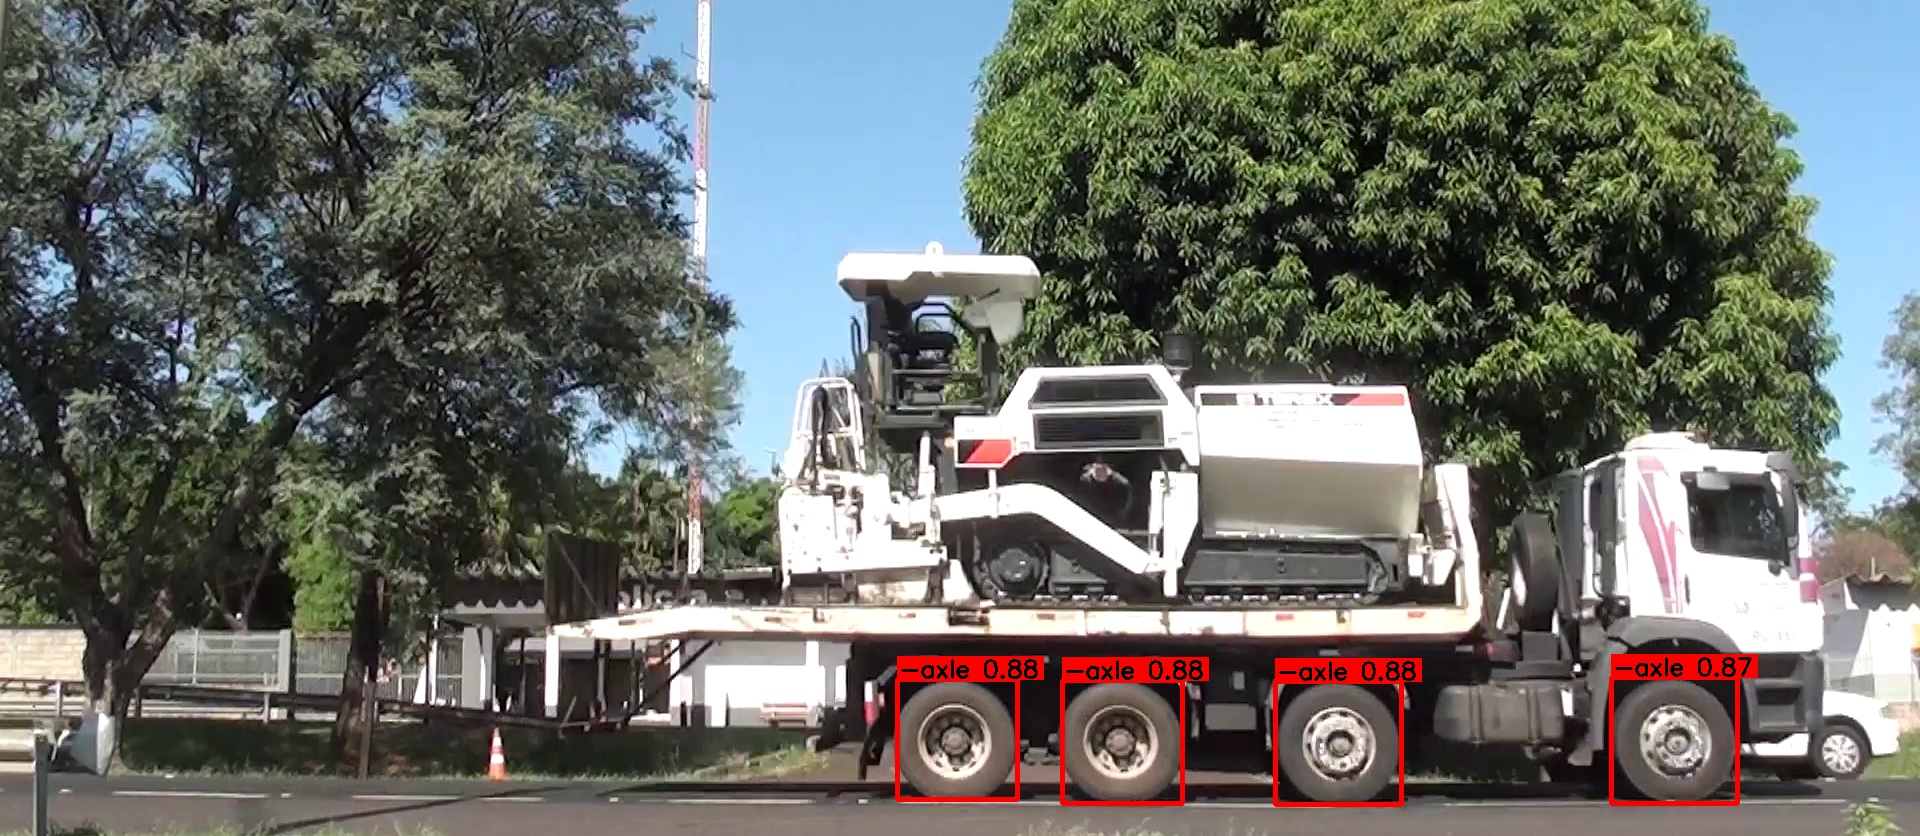
\includegraphics[width=1\linewidth]{Images//yolo_outputs/yolo_output_20170418095402_color-[ROI-1]-94(1).jpg}
            \caption{Predição pelo modelo YOLOv11 com caminhão de quatro eixos}
            \label{fig:predicao_yolo_1}
        \end{figure}

        \begin{figure} [!htb]
            \centering
            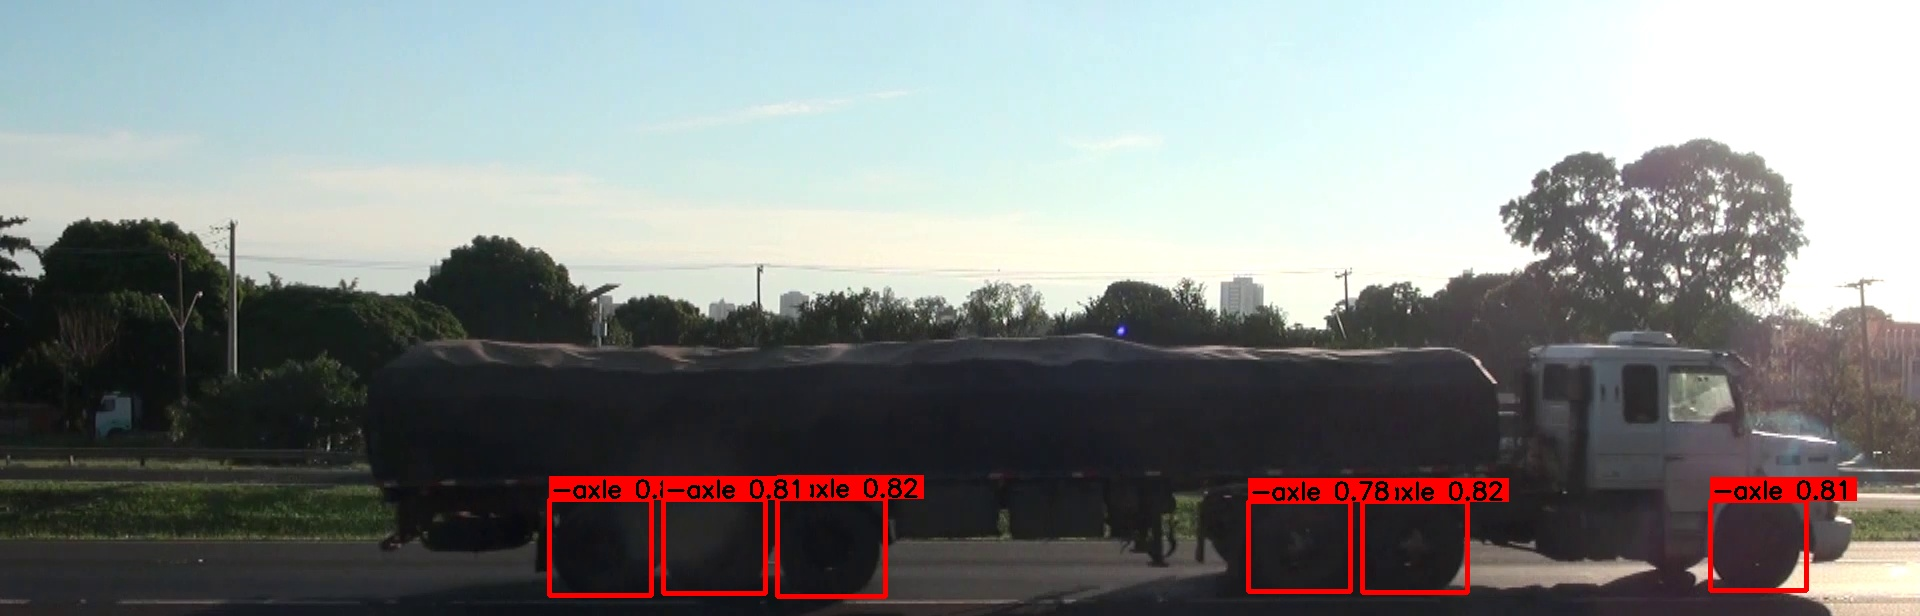
\includegraphics[width=1\linewidth]{Images//yolo_outputs/yolo_output_20170418074140-550_color-[ROI-1]-30.jpg}
            \caption{Predição pelo modelo YOLOv11 com caminhão de seis eixos}
            \label{fig:predicao_yolo_2}
        \end{figure}

        \begin{figure} [!htb]
            \centering
            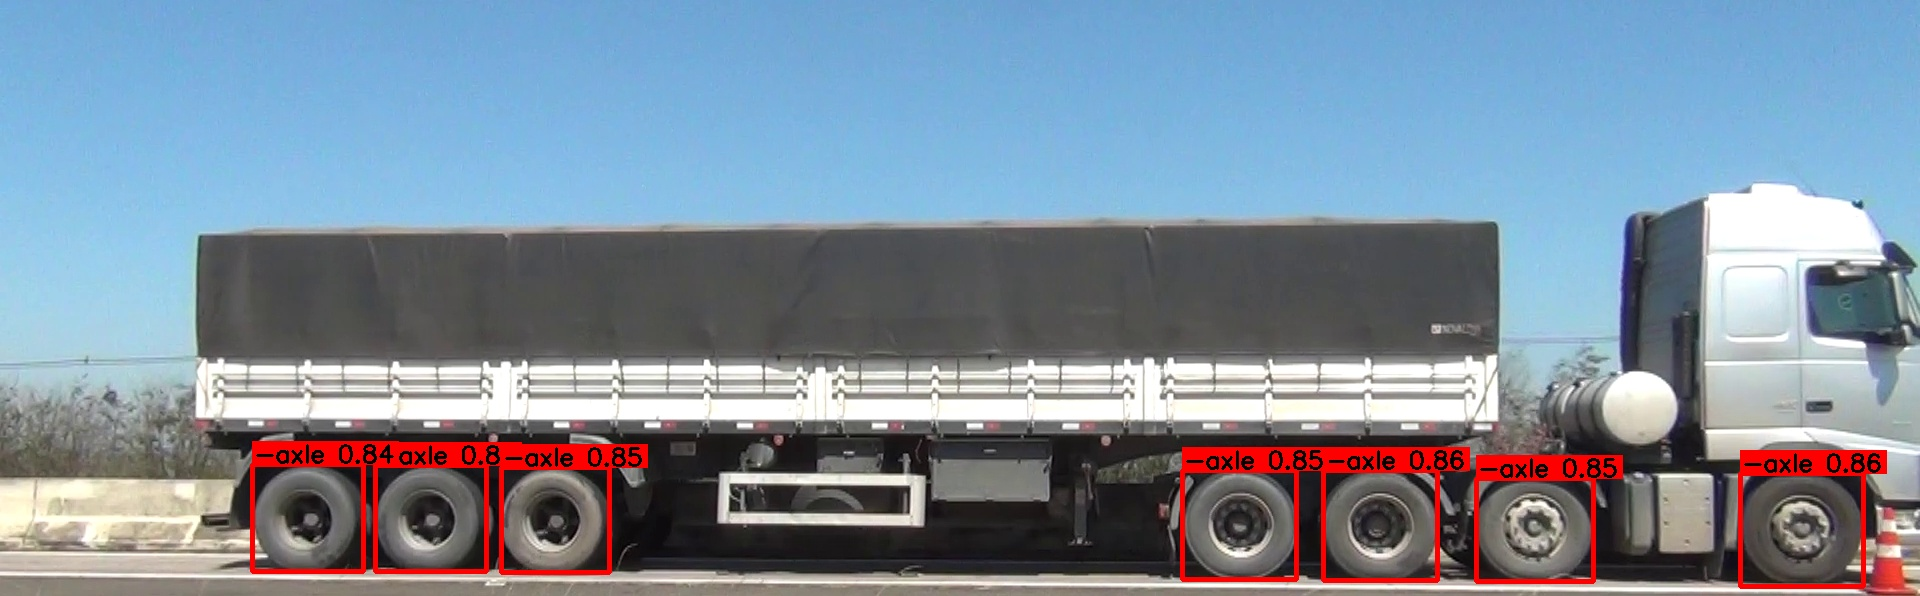
\includegraphics[width=1\linewidth]{Images//yolo_outputs/yolo_output_20160927102749_color-[ROI-1]-1.jpg}
            \caption{Predição pelo modelo YOLOv11 com caminhão de sete eixos}
            \label{fig:predicao_yolo_3}
        \end{figure}
        
    \subsection{Modelos de contagem}
        Para os modelos de regressão que realizam a contagem de eixos, foram analisados dois modelos para transferência de aprendizado, a InceptionV3 (utilizada em \cite{Almutairi2022}) e a ResNet152 (uma versão mais robusta da utilizada em \cite{iluminacao_adversa}), uma vez que mostraram bons desempenhos em tarefas semelhantes envolvendo veículos.

        A estrutura dos modelos é a mesma para ambos e pode ser vista na figura \ref{fig:modelo_base}. A entrada corresponde a uma imagem RGB de 640x640 pixeis, alimentando as redes InceptionV3 e a ResNet, que se conectam a uma camada densa com 512 neurônios e ativação ReLU, seguida de uma camada densa com 256 neurônios, ativação ReLU e BatchNormalization, depois há uma camada densa com 32 neurônios e ativação ReLU, e, por fim, uma camada densa com um neurônio, mas sem ativação.

        \begin{figure}[!htb]
            \centering
            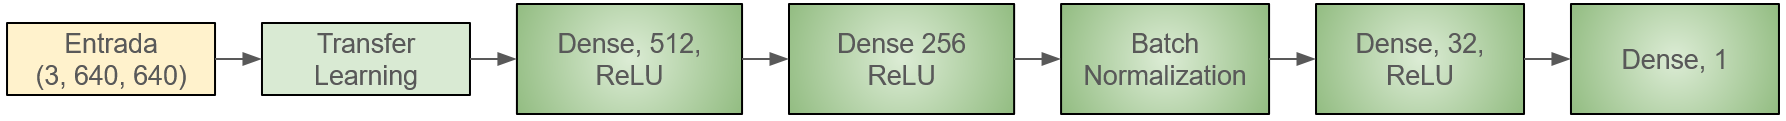
\includegraphics[width=1\linewidth]{Images/modelo.png}
            \caption{Modelo base}
            \label{fig:modelo_base}
        \end{figure}

        Os modelos foram treinados utilizando o otimizador SGD, com \textit{learning rate} de 0.001 e \textit{momentum} de 0.9, tendo como função de erro a Mean Squared Error (MSE). O treinamento poderia ser realizado por até 25 épocas; no entanto, para mitigar o risco de \textit{overfitting}, foi implementado um mecanismo de \textit{Early Stopping} com paciência de três épocas, monitorando o erro de validação como critério de interrupção.
        
        Após o treinamento, os modelos foram avaliados utilizando o conjunto de teste. Para cada imagem, foi realizada uma predição, cujo resultado foi arredondado. A partir desses valores, foram calculadas a precisão, o \textit{recall}, o F1 Score e a acurácia de cada modelo. Além disso, os modelos baseados na YOLO também foram comparados, considerando apenas a quantidade de eixos identificados, sem levar em conta sua localização.
    
        \begin{table}[!htb]
            \begin{tabular}{| c | c | c | c | c | c | c |}
                \hline
                Modelo      & Precision & Recall & F1 Score & Acurácia & Teste loss & MAE Loss \\
                \hline
                ResNet152 & 0.85 & 0.87 & 0.85 & 0.91 & 0.10 & 0.24 \\
                InceptionV3 & 0.88 & 0.85 & 0.86 & 0.92 & 0.12 & 0.22 \\
                YOLOv11m & 0.93 & 0.95 & 0.94 & 0.96 & 0.06 & 0.05    \\
                YOLOv12m & 0.91 & 0.92 & 0.92 & 0.94 & 0.08 & 0.06 \\
                \hline
            \end{tabular}
            \caption{Avaliação dos modelos}
            \label{tab:avaliacao}
        \end{table}

        A tabela \ref{tab:avaliacao} apresenta os resultados obtidos da avaliação dos modelos. Dessa forma, percebe-se que o modelo implementado com a YOLOv11 supera os demais, mesmo que ainda apresentem resultados competitivos, principalmente a InceptionV3 e a YOLOv12. 

        Realizando as predições para as mesmas imagens que geraram as saídas vistas nas figuras \ref{fig:predicao_yolo_1}, \ref{fig:predicao_yolo_2} e \ref{fig:predicao_yolo_3}, obteve-se as predições vistas na tabela \ref{tab:predicao}.        

        \begin{table} [!htb]
            \centering
            \begin{tabular}{| c | c | c | c | c |}
            \hline
            Imagem               & Modelo      & Predição & Arredondamento & Valor real          \\
            \hline
            \multirow{4}{*}{Figura \ref{fig:predicao_yolo_1}} & ResNet      & 6.30     & 6              & \multirow{4}{*}{7}  \\
                                 & InceptionV3 & 5.95     & 6              &                     \\
                                 & YOLOv11m    & 7        & 7              &                     \\
                                 & YOLOv12m    & 7        & 7              &                     \\
            \hline
            \multirow{4}{*}{Figura \ref{fig:predicao_yolo_2}}   & ResNet      & 5.71     & 6              & \multirow{4}{*}{6}  \\
                                 & InceptionV3 & 5.80     & 6              &                     \\
                                 & YOLOv11m    & 6        & 6              &                     \\
                                 & YOLOv12m    & 6        & 6              &                     \\
            \hline
            \multirow{4}{*}{Figura \ref{fig:predicao_yolo_3}}   & ResNet      & 4.01     & 4              & \multirow{4}{*}{4}  \\
                                 & InceptionV3 & 3.76     & 4              &                     \\
                                 & YOLOv11m    & 4        & 4              &                     \\      & YOLOv12m    & 4        & 4              &                     \\                    
            \hline
            \end{tabular}
            \caption{Predição dos modelos}
            \label{tab:predicao}
        \end{table}

        Assim, com tais resultados que corroboram com os dados vistos na tabela \ref{tab:avaliacao}, percebe-se que o uso da YOLOv11 é mais atrativo até mesmo para a tarefa de contagem de eixos. Ademais, o seu custo computacional inferior aos modelos que usam CNN's fazem com que o seu uso seja ainda mais adequado, mesmo no contexto em que, segundo o seu artigo, a YOLOv12 possa ser mais rápida.
            
\section{Conclusão}
    A partir de testes com diferentes arquiteturas e modelos, foi possível identificar uma configuração que se destacou em relação às demais, apresentando alta taxa de acertos e menor custo computacional. Tal modelo é o que foi refinado a partir da YOLOv11m, alcançando um F1 Score de 0.99 na detecção de eixos. No entanto, os valores do mAP50-95 ainda podem ser aprimorados por meio de uma definição mais precisa das \textit{bounding boxes} nas imagens.

    Para trabalhos futuros, seria interessante considerar o uso de imagens capturadas em períodos noturnos, bem como explorar modelos capazes de diferenciar distintos veículos na cena, em vez de agrupá-los como um único objeto. Essa abordagem seria essencial para a implementação de um sistema em tempo real capaz de lidar com múltiplos veículos simultaneamente.


\section{Código fonte}
    O código fonte utilizado no trabalho pode ser encontrado no \href{https://github.com/matheusprv/truck-axle-detection}{Repositório do projeto}.

\section{Referências}
\bibliographystyle{sbc}

\bibliography{sbc-template}

\end{document}
